\input{../cs164.tex}
\usepackage{amsmath, verbatim, tikz, float}

\usetikzlibrary{arrows,automata}

\oddsidemargin 0in
\evensidemargin 0in
\textwidth 6.5in
\topmargin -0.5in
\textheight 9.0in
\newcommand{\norm}[1]{\left\lVert #1 \right\rVert}
\newcommand{\?}{\stackrel{?}{=}}

\begin{document}

\solution{Nikhil Unni (cs164-es)}{WA1}{Fall 2015}
\pagestyle{myheadings}


\begin{enumerate}
    \item Give a DFA for the following languages over the alphabet $\Sigma = \{a,b\}$:
    \begin{itemize}
      \item All strings that contain at most two a's.\\
        \begin{figure}[H]
        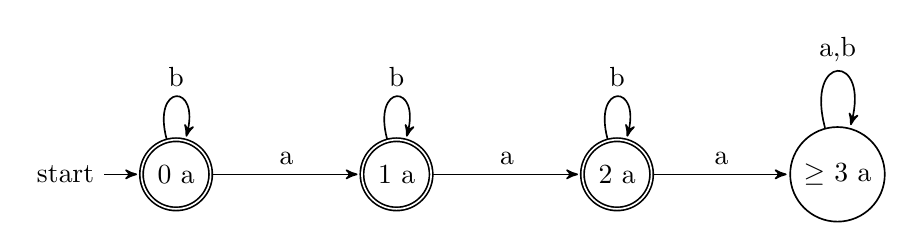
\begin{tikzpicture}[->,>=stealth',shorten >=1pt,auto,node distance=2.8cm, semithick]
          \tikzstyle{every state}=[fill=none,draw=black,text=black]
          \node[initial,state,accepting] (A)              {0 a};
          \node[state,accepting]         (B) [right of=A] {1 a};
          \node[state,accepting]         (C) [right of=B] {2 a};
          \node[state]                   (D) [right of=C] {$\geq$ 3 a};

          \path (A) edge              node {a}   (B)
                    edge [loop above] node {b}   (A)
                (B) edge              node {a}   (C)
                    edge [loop above] node {b}   (B)
                (C) edge              node {a}   (D)
                    edge [loop above] node {b}   (C)
                (D) edge [loop above] node {a,b} (D);
        \end{tikzpicture}
        \end{figure}
      \item All strings that contain at most one b.\\
        \begin{figure}[H]
        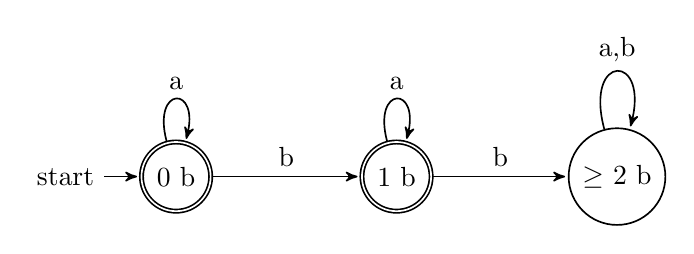
\begin{tikzpicture}[->,>=stealth',shorten >=1pt,auto,node distance=2.8cm, semithick]
          \tikzstyle{every state}=[fill=none,draw=black,text=black]
          \node[initial,state,accepting] (A)              {0 b};
          \node[state,accepting]         (B) [right of=A] {1 b};
          \node[state]                   (C) [right of=B] {$\geq$ 2 b};

          \path (A) edge              node {b}   (B)
                    edge [loop above] node {a}   (A)
                (B) edge              node {b}   (C)
                    edge [loop above] node {a}   (B)
                (C) edge [loop above] node {a,b} (C);
        \end{tikzpicture}
        \end{figure}
      \item All strings that contain at most two a's and at most one b.\\
        \begin{figure}[H]
        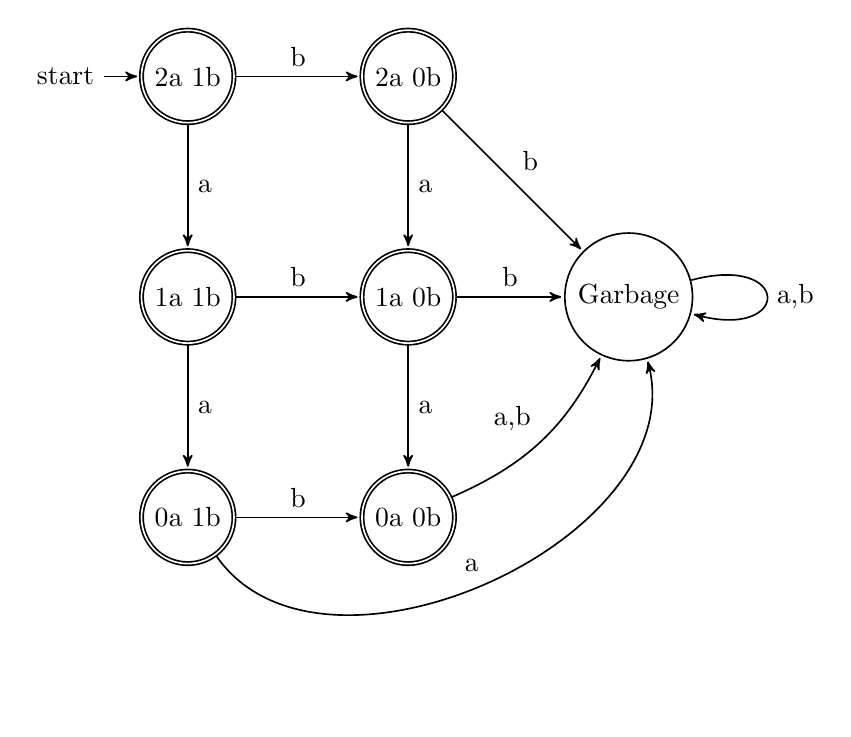
\begin{tikzpicture}[->,>=stealth',shorten >=1pt,auto,node distance=2.8cm, semithick]
          \tikzstyle{every state}=[fill=none,draw=black,text=black]
          \node[initial,state,accepting] (A)              {2a 1b};
          \node[state,accepting]         (B) [right of=A] {2a 0b};
          \node[state,accepting]         (C) [below of=A] {1a 1b};
          \node[state,accepting]         (D) [right of=C] {1a 0b};
          \node[state,accepting]         (E) [below of=C] {0a 1b};
          \node[state,accepting]         (F) [right of=E] {0a 0b};
          \node[state]                   (G) [right of=D] {Garbage};

          \path (A) edge                 node {b}   (B)
                    edge                 node {a}   (C)
                (B) edge                 node {b}   (G)
                    edge                 node {a}   (D)
                (C) edge                 node {b}   (D)
                    edge                 node {a}   (E)
                (D) edge                 node {b}   (G)
                    edge                 node {a}   (F)
                (E) edge                 node {b}   (F)
                    edge [bend right=80] node {a}   (G)
                (F) edge [bend right=20] node {a,b} (G)
                (G) edge [loop right]    node {a,b} (G);
        \end{tikzpicture}
        \end{figure}
      \item All strings that contain at least one a and no b's.\\
        \begin{figure}[H]
        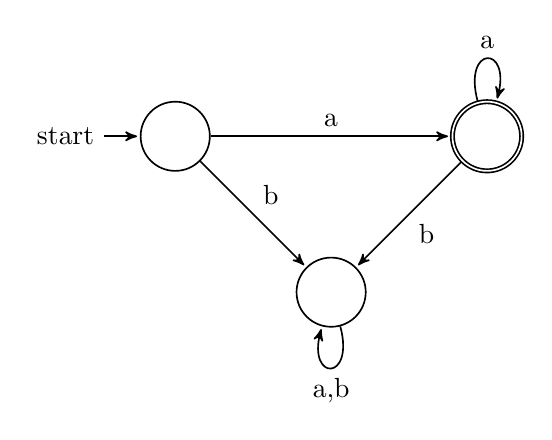
\begin{tikzpicture}[->,>=stealth',shorten >=1pt,auto,node distance=2.8cm, semithick]
          \tikzstyle{every state}=[fill=none,draw=black,text=black]
          \node[initial,state]    (A)                    {};
          \node[state]            (B) [below right of=A] {};
          \node[state,accepting]  (C) [above right of=B] {};

          \path (A) edge              node {a}   (C)
                    edge              node {b}   (B)
                (B) edge [loop below] node {a,b} (B)
                (C) edge [loop above] node {a}   (C)
                    edge              node {b}   (B);
        \end{tikzpicture}
        \end{figure}

    \end{itemize}
  \item Consider the following DFA over the alphabet $\Sigma = \{a,b\}$. (Not pictured.)\\
    Give a one sentence description of the language recognized by the DFA. Write a regular expression for the same language.\\\\

    It is the set of words where the number of a's is divisible by 4. It can be represented by the regex $(b^*ab^*ab^*ab^*ab^*)^*$.
  \item Let $\Sigma_m = \{a_1, \cdots, a_m\}$ be an alphabet containing $m$ elements, for some integer $m \geq 2$. Let $L_m$ be the following language that includes all strings in which at least one of the characters occurs an odd number of times and one of the characters occurs an even number of times.\\\\

    Construct a DFA for the language $L_2$.
        \begin{figure}[H]
        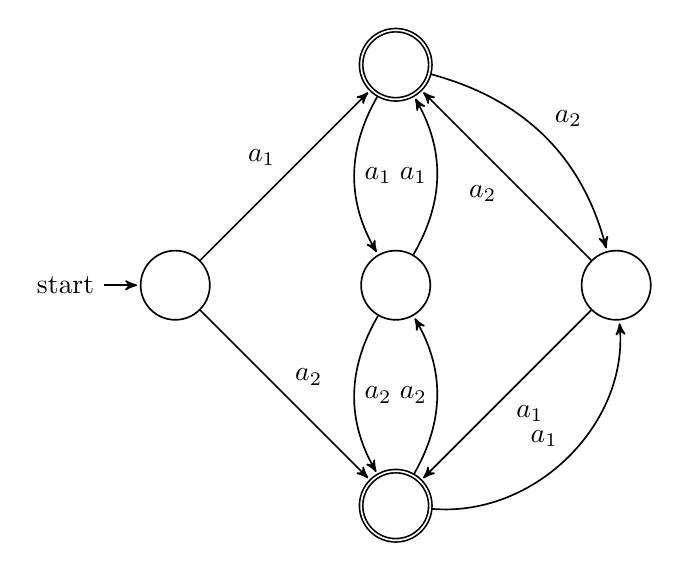
\begin{tikzpicture}[->,>=stealth',shorten >=1pt,auto,node distance=2.8cm, semithick]
          \tikzstyle{every state}=[fill=none,draw=black,text=black]
          \node[initial,state]   (A)              {};
          \node[state]           (B) [right of=A] {};
          \node[state]           (C) [right of=B] {};
          \node[state,accepting] (D) [above of=B] {};
          \node[state,accepting] (E) [below of=B] {};

          \path (A) edge node {$a_1$} (D)
                    edge node {$a_2$} (E)
                (B) edge [bend right=30] node {$a_1$} (D)
                    edge [bend right=30] node {$a_2$} (E)
                (C) edge node {$a_2$} (D)
                    edge node {$a_1$} (E)
                (D) edge [bend right=30] node {$a_1$} (B)
                    edge [bend left=30] node {$a_2$} (C)
                (E) edge [bend right=30] node {$a_2$} (B)
                    edge [bend right=50] node {$a_1$} (C);

        \end{tikzpicture}
        \end{figure}
    Also construct an NFA for the language $L_3$.    
        \begin{figure}[H]
        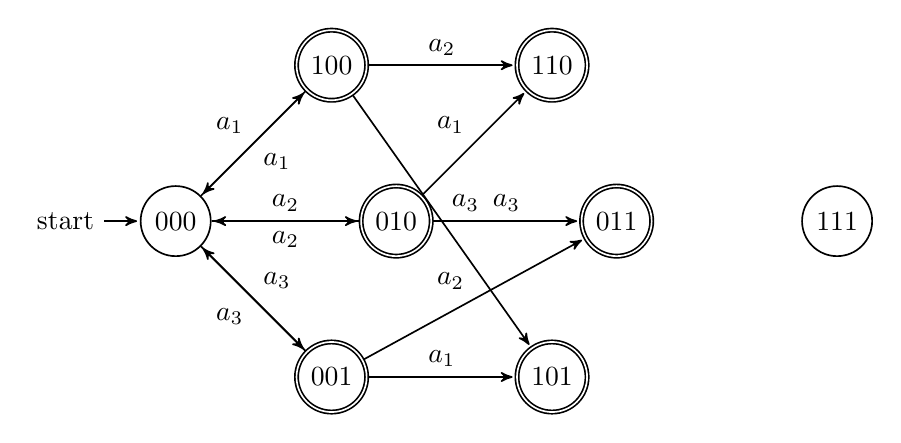
\begin{tikzpicture}[->,>=stealth',shorten >=1pt,auto,node distance=2.8cm, semithick]
          \tikzstyle{every state}=[fill=none,draw=black,text=black]
          \node[initial,state]   (A)                    {000};
          \node[state,accepting] (B) [above right of=A] {100};
          \node[state,accepting] (C) [right of=A]       {010};
          \node[state,accepting] (D) [below right of=A] {001};
          \node[state,accepting] (E) [right of=B]       {110};
          \node[state,accepting] (F) [right of=D]       {101};
          \node[state,accepting] (G) [right of=C]       {011};
          \node[state]           (H) [right of=G]       {111};

          \path (A) edge node {$a_1$} (B)
                    edge node {$a_2$} (C)
                    edge node {$a_3$} (D)
                (B) edge node {$a_1$} (A)
                    edge node {$a_2$} (E)
                    edge node {$a_3$} (F)
                (C) edge node {$a_1$} (E)
                    edge node {$a_2$} (A)
                    edge node {$a_3$} (G)
                (D) edge node {$a_1$} (F)
                    edge node {$a_2$} (G)
                    edge node {$a_3$} (A);

        \end{tikzpicture}
        \end{figure}

\end{enumerate}

\end{document}
